\documentclass[a4paper,12pt]{article}

% ---------- Packages ----------
\usepackage[utf8]{inputenc}
\usepackage[T1]{fontenc}
\usepackage{lmodern}
\usepackage[margin=2.5cm]{geometry}
\usepackage{hyperref}
\usepackage{xcolor}
\usepackage{listings}
\usepackage{enumitem}
\usepackage{booktabs}
\usepackage{array}
\usepackage{longtable}
\usepackage{fancyhdr}
\usepackage{titlesec}
\usepackage{parskip}
\usepackage{graphicx}
\usepackage{mdframed}
\usepackage{amsmath}
\usepackage{amssymb}
\usepackage{tikz}
\usetikzlibrary{calc}
\usepackage{graphicx}
\usepackage{tcolorbox}
\tcbuselibrary{skins,breakable}

% ---------- Hyperlink setup ----------
\hypersetup{
    colorlinks=true,
    linkcolor=blue!70!black,
    urlcolor=blue!70!black,
    citecolor=blue!70!black,
    pdftitle={Accessing Debian XFCE on Windows Client},
    pdfauthor={Remote Desktop Setup Guide},
}

% ---------- Header / Footer ----------
\pagestyle{fancy}
\fancyhf{}
\fancyhead[L]{\small Accessing Debian XFCE on Windows Client}
\fancyhead[R]{\small\thepage}
\renewcommand{\headrulewidth}{0.4pt}
\renewcommand{\footrulewidth}{0pt}

% ---------- Code listing styles ----------
\definecolor{codebg}{RGB}{245,245,245}
\definecolor{codeframe}{RGB}{200,200,200}
\definecolor{codecomment}{RGB}{0,128,0}
\definecolor{codekeyword}{RGB}{0,0,255}
\definecolor{codestring}{RGB}{163,21,21}
\definecolor{codegray}{RGB}{128,128,128}
\definecolor{notebg}{RGB}{255,250,205}
\definecolor{noteframe}{RGB}{218,165,32}
\definecolor{tipbg}{RGB}{230,245,230}
\definecolor{tipframe}{RGB}{60,140,60}
\definecolor{warnbg}{RGB}{255,235,235}
\definecolor{warnframe}{RGB}{200,60,60}

\lstdefinestyle{bashstyle}{
    backgroundcolor=\color{codebg},
    frame=single,
    rulecolor=\color{codeframe},
    basicstyle=\ttfamily\small,
    keywordstyle=\color{codekeyword}\bfseries,
    commentstyle=\color{codecomment}\itshape,
    stringstyle=\color{codestring},
    numbers=none,
    numberstyle=\tiny\color{codegray},
    breaklines=true,
    breakatwhitespace=false,
    postbreak=\mbox{\textcolor{red}{$\hookrightarrow$}\space},
    showstringspaces=false,
    tabsize=4,
    columns=flexible,
    keepspaces=true,
    xleftmargin=1em,
    xrightmargin=1em,
    aboveskip=1em,
    belowskip=1em,
}

\lstdefinestyle{textstyle}{
    backgroundcolor=\color{codebg},
    frame=single,
    rulecolor=\color{codeframe},
    basicstyle=\ttfamily\small,
    breaklines=true,
    postbreak=\mbox{\textcolor{red}{$\hookrightarrow$}\space},
    showstringspaces=false,
    tabsize=4,
    columns=flexible,
    keepspaces=true,
    xleftmargin=1em,
    xrightmargin=1em,
    aboveskip=1em,
    belowskip=1em,
}

\lstdefinestyle{shstyle}{
    backgroundcolor=\color{codebg},
    frame=single,
    rulecolor=\color{codeframe},
    basicstyle=\ttfamily\small,
    keywordstyle=\color{codekeyword}\bfseries,
    commentstyle=\color{codecomment}\itshape,
    stringstyle=\color{codestring},
    language=bash,
    breaklines=true,
    postbreak=\mbox{\textcolor{red}{$\hookrightarrow$}\space},
    showstringspaces=false,
    tabsize=4,
    columns=flexible,
    keepspaces=true,
    xleftmargin=1em,
    xrightmargin=1em,
    aboveskip=1em,
    belowskip=1em,
}

\lstset{style=bashstyle}

% ---------- Custom command for inline code ----------
\newcommand{\code}[1]{\texttt{\small #1}}

% ---------- Custom boxes ----------
\newtcolorbox{notebox}{
    colback=notebg,
    colframe=noteframe,
    boxrule=0.8pt,
    arc=3pt,
    left=6pt,
    right=6pt,
    top=4pt,
    bottom=4pt,
    breakable,
    title={\bfseries Note},
    fonttitle=\bfseries,
}

\newtcolorbox{tipbox}{
    colback=tipbg,
    colframe=tipframe,
    boxrule=0.8pt,
    arc=3pt,
    left=6pt,
    right=6pt,
    top=4pt,
    bottom=4pt,
    breakable,
    title={\bfseries Tip},
    fonttitle=\bfseries,
}

\newtcolorbox{warnbox}{
    colback=warnbg,
    colframe=warnframe,
    boxrule=0.8pt,
    arc=3pt,
    left=6pt,
    right=6pt,
    top=4pt,
    bottom=4pt,
    breakable,
    title={\bfseries Warning},
    fonttitle=\bfseries,
}

% ---------- Section title formatting ----------
\titleformat{\section}
    {\Large\bfseries\color{blue!70!black}}
    {\thesection}{1em}{}
\titleformat{\subsection}
    {\large\bfseries\color{blue!60!black}}
    {\thesubsection}{1em}{}
\titleformat{\subsubsection}
    {\normalsize\bfseries\color{blue!50!black}}
    {\thesubsubsection}{1em}{}

% ---------- Document ----------
\begin{document}

% ============================================================
% TITLE PAGE
% ============================================================
% ============================================================
% FULL-PAGE COVER IMAGE
% ============================================================
\begin{titlepage}
	\thispagestyle{empty}
	\centering
	% Remove default margins locally so image fills the page
	\begin{tikzpicture}[remember picture, overlay]
		\node[inner sep=0pt] at (current page.center) {%
			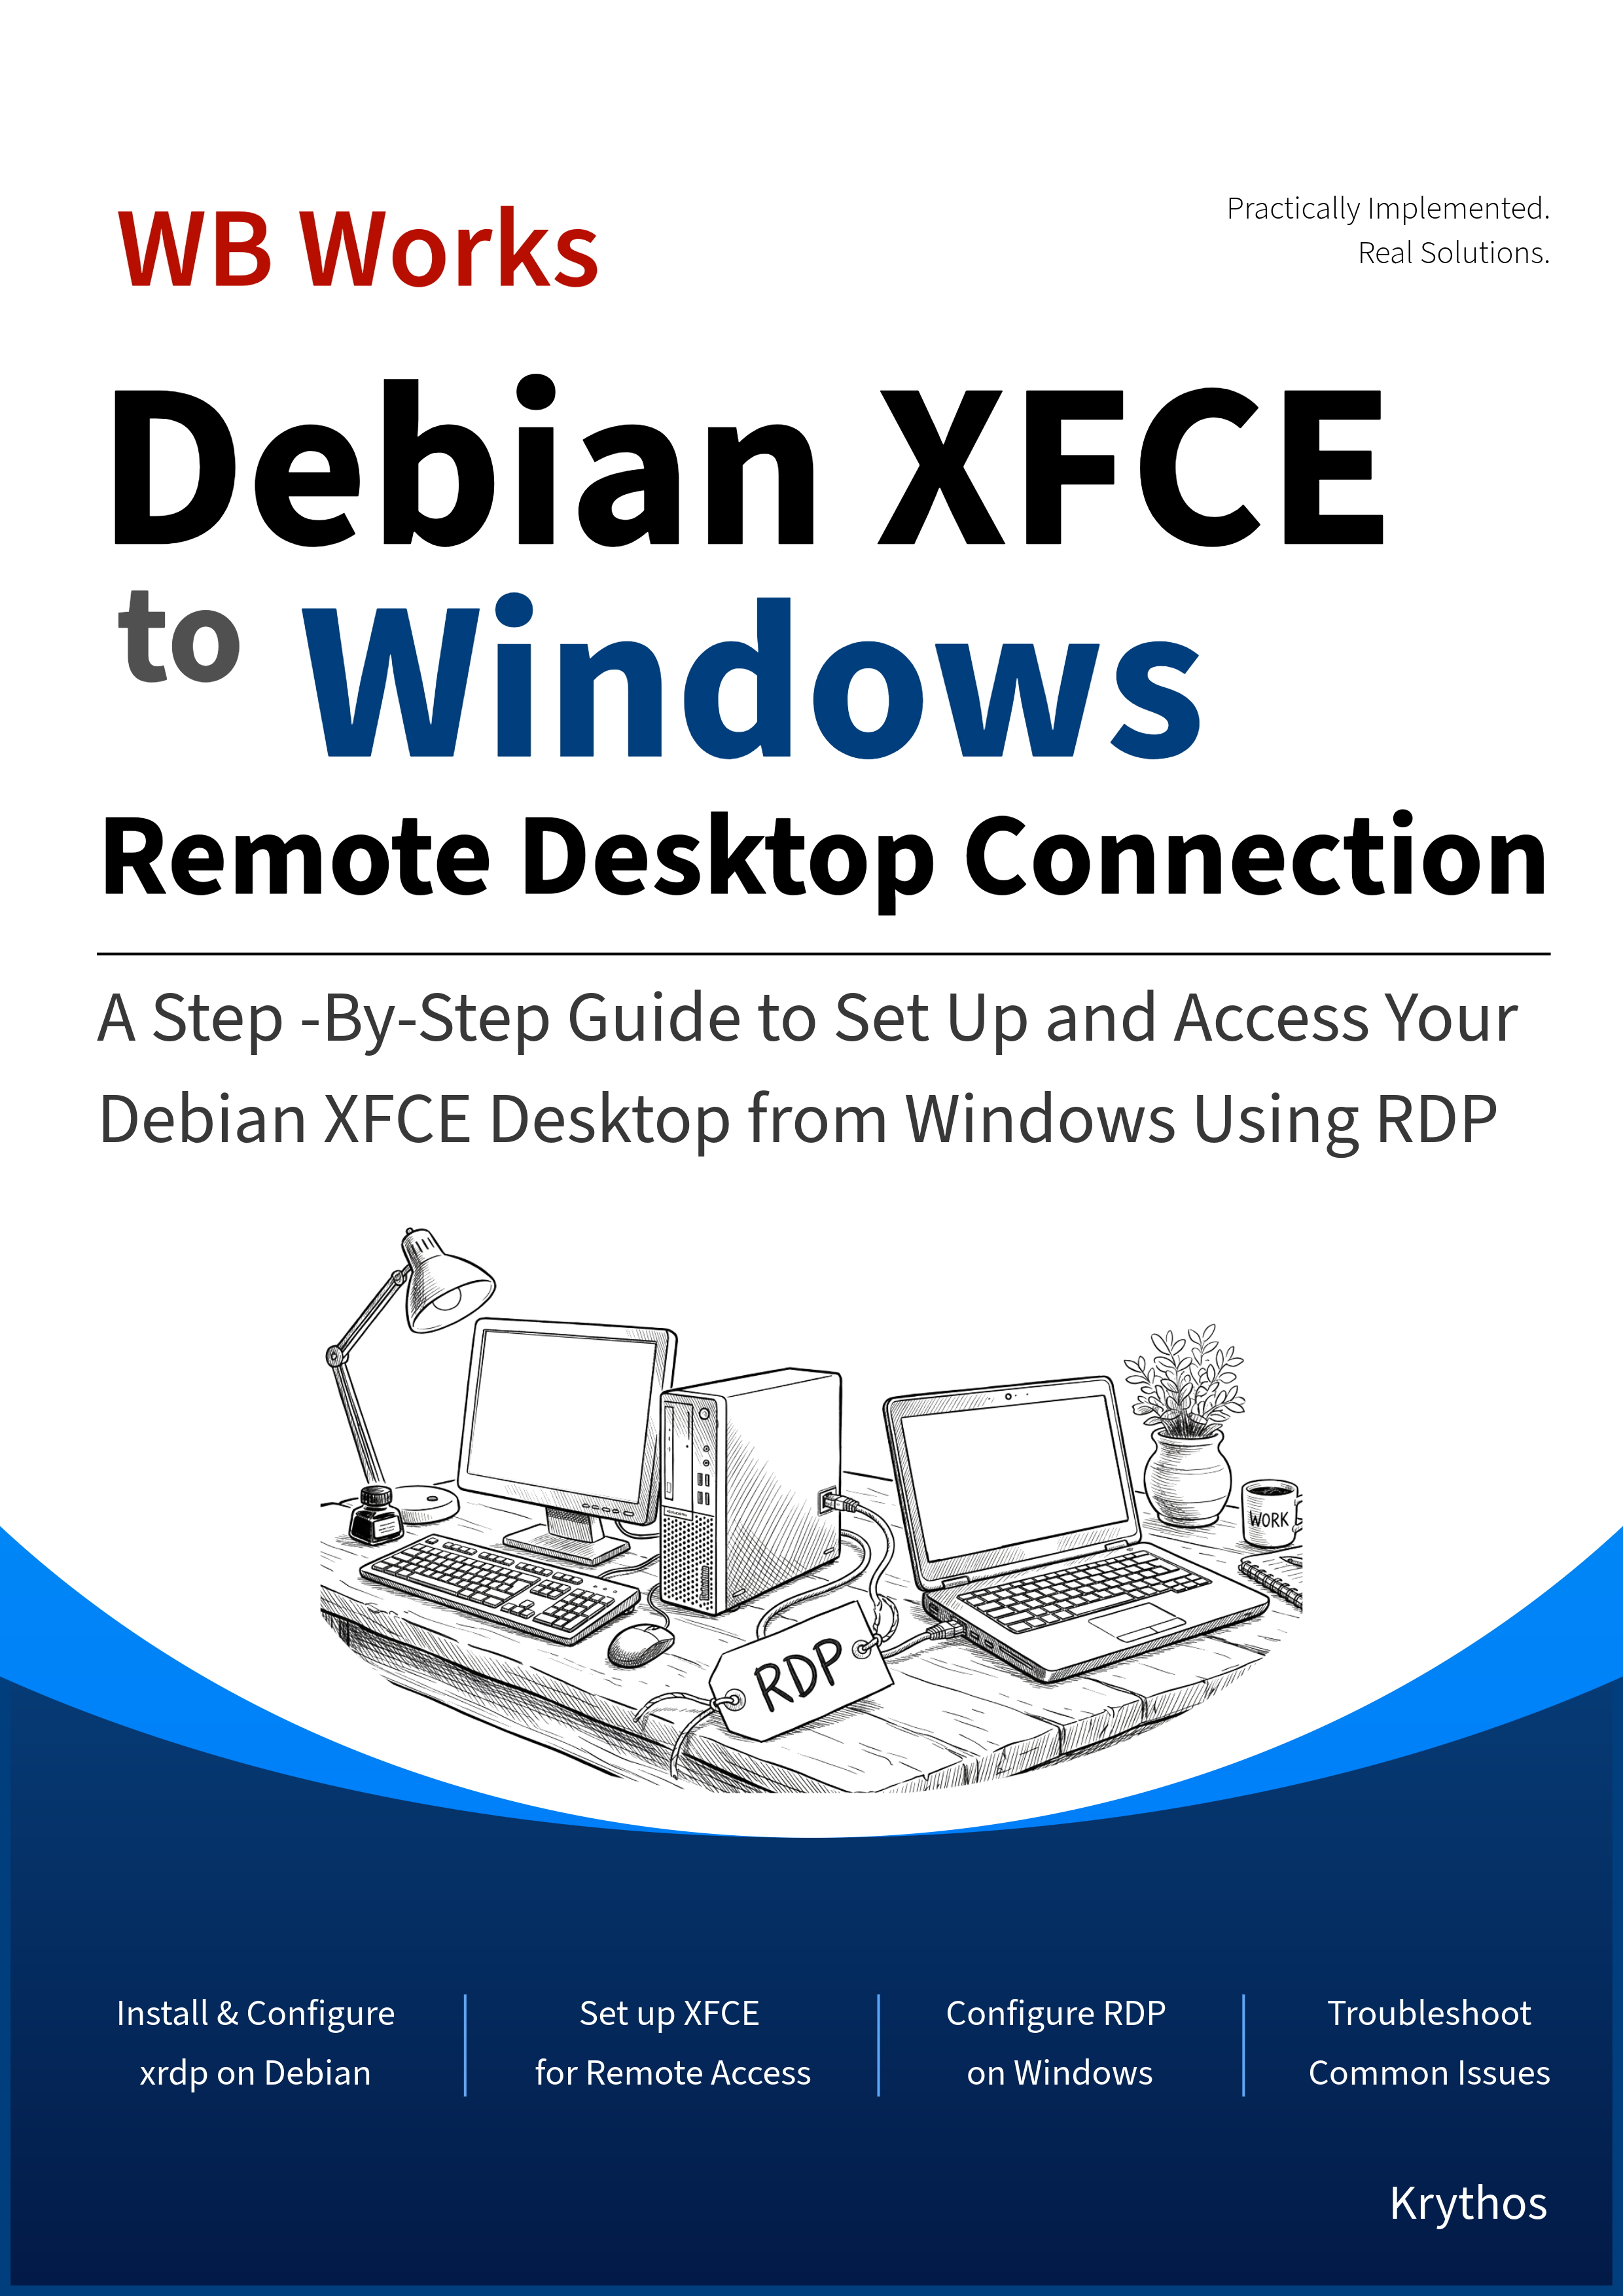
\includegraphics[width=\paperwidth,height=\paperheight]{cover page.png}%
		};
	\end{tikzpicture}
	\null
\end{titlepage}

% ============================================================
% TABLE OF CONTENTS
% ============================================================
\newpage
\tableofcontents
\newpage

% ============================================================
\section{Introduction}
% ============================================================

This guide explains how to access a \textbf{Debian 13 XFCE} desktop from a \textbf{Windows 11} PC using the built-in \textbf{Remote Desktop Connection} client (\code{mstsc.exe}).

The setup uses \textbf{XRDP}, which is a free and open-source RDP server for Linux. It allows you to create a \textbf{separate graphical XFCE session} on the Debian machine that is independent of the physical desktop.

\subsection{What You Will Achieve}

After following this guide:

\begin{itemize}[leftmargin=2em]
    \item The Debian PC (PC1) will run an XRDP server.
    \item The Windows PC (PC2) will connect to PC1 using Remote Desktop.
    \item You will see a \textbf{new, separate XFCE desktop} inside the Windows RDP window.
    \item The physical Debian desktop (if someone is sitting at it) will remain active and unaffected.
\end{itemize}

\subsection{Architecture Overview}

\begin{lstlisting}[style=textstyle]
+-----------------------------+          +-----------------------------+
|        PC2 (Windows 11)     |          |      PC1 (Debian 13)        |
|                             |          |                             |
|   mstsc.exe                 |   RDP    |   xrdp (TCP 3389)           |
|   Remote Desktop Client     | -------> |   xrdp-sesman               |
|                             |          |   Xorg :10                  |
|   192.168.1.14              |          |   XFCE Session              |
|                             |          |   192.168.1.9               |
+-----------------------------+          +-----------------------------+
\end{lstlisting}

\begin{notebox}
The IP addresses \code{192.168.1.14} and \code{192.168.1.9} are examples. Replace them with the actual IP addresses of your own machines.
\end{notebox}

% ============================================================
\section{Prerequisites}
% ============================================================

Before starting, ensure the following:

\begin{enumerate}[leftmargin=2em]
    \item \textbf{PC1 (Debian 13 XFCE)} is installed and working with a graphical desktop.
    \item \textbf{PC2 (Windows 11)} is installed and working.
    \item Both PCs are connected to the \textbf{same local network} (LAN/Wi-Fi).
    \item You know the \textbf{username and password} for the Debian account you will use.
    \item You have \textbf{sudo/root} access on the Debian PC.
    \item You know the \textbf{IP address} of the Debian PC.
\end{enumerate}

\begin{tipbox}
If you are unsure about the Debian IP address, you can find it later in Section~4. For now, just make sure both machines are on the same network.
\end{tipbox}

% ============================================================
\section{Understanding XRDP}
% ============================================================

XRDP is an open-source implementation of the Microsoft RDP protocol. It allows a Linux machine to accept connections from any standard RDP client, including the one built into Windows.

\subsection{How the Connection Works}

\begin{lstlisting}[style=textstyle]
Windows mstsc
       |
       | RDP (TCP 3389)
       v
     xrdp
       |
       v
  xrdp-sesman
       |
       v
      Xorg
       |
       v
 XFCE Session
\end{lstlisting}

\subsection{Key Components}

\begin{itemize}[leftmargin=2em]
    \item \code{xrdp} --- The main service that listens for incoming RDP connections on port 3389.
    \item \code{xrdp-sesman} --- The session manager that creates and manages the graphical session.
    \item \code{Xorg} / \code{xorgxrdp} --- Provides the virtual X display for the RDP session.
    \item \code{startxfce4} --- The command that starts the XFCE desktop.
    \item \code{dbus-run-session} --- Ensures the RDP session gets its own DBus session, which is required for XFCE to start correctly.
\end{itemize}

% ============================================================
\section{Step 1 --- Find the Debian PC's IP Address}
% ============================================================

On \textbf{PC1 (Debian)}, open a terminal and run:

\begin{lstlisting}[style=bashstyle]
hostname -I
\end{lstlisting}

Alternatively, you can use:

\begin{lstlisting}[style=bashstyle]
ip addr
\end{lstlisting}

Look for an address like:

\begin{lstlisting}[style=textstyle]
192.168.1.9
\end{lstlisting}

\begin{notebox}
Write this IP address down. You will need it when connecting from Windows. In this guide, we will use \code{192.168.1.9} as the example Debian IP.
\end{notebox}

% ============================================================
\section{Step 2 --- Update Debian}
% ============================================================

On \textbf{PC1 (Debian)}, open a terminal and update the package lists:

\begin{lstlisting}[style=bashstyle]
sudo apt update
\end{lstlisting}

Optionally, upgrade installed packages:

\begin{lstlisting}[style=bashstyle]
sudo apt upgrade -y
\end{lstlisting}

\begin{tipbox}
Keeping your system updated ensures you get the latest security patches and package versions.
\end{tipbox}

% ============================================================
\section{Step 3 --- Install XRDP and Required Packages}
% ============================================================

\subsection{Install XRDP}

\begin{lstlisting}[style=bashstyle]
sudo apt install xrdp -y
\end{lstlisting}

\subsection{Install DBus Support}

XRDP requires DBus to create a proper desktop session:

\begin{lstlisting}[style=bashstyle]
sudo apt install dbus-x11 -y
\end{lstlisting}

\subsection{Verify XFCE Is Installed}

Most Debian XFCE installations already have XFCE. Verify:

\begin{lstlisting}[style=bashstyle]
command -v startxfce4
\end{lstlisting}

Expected output:

\begin{lstlisting}[style=textstyle]
/usr/bin/startxfce4
\end{lstlisting}

If the command is not found, install XFCE:

\begin{lstlisting}[style=bashstyle]
sudo apt install xfce4 xfce4-goodies -y
\end{lstlisting}

\subsection{Verify dbus-run-session}

\begin{lstlisting}[style=bashstyle]
command -v dbus-run-session
\end{lstlisting}

Expected output:

\begin{lstlisting}[style=textstyle]
/usr/bin/dbus-run-session
\end{lstlisting}

If it is missing, reinstall \code{dbus-x11}:

\begin{lstlisting}[style=bashstyle]
sudo apt install --reinstall dbus-x11 -y
\end{lstlisting}

% ============================================================
\section{Step 4 --- Enable and Start the XRDP Service}
% ============================================================

Enable XRDP to start automatically at boot and start it immediately:

\begin{lstlisting}[style=bashstyle]
sudo systemctl enable --now xrdp
\end{lstlisting}

\subsection{Check the Service Status}

\begin{lstlisting}[style=bashstyle]
systemctl status xrdp
\end{lstlisting}

You should see:

\begin{lstlisting}[style=textstyle]
Active: active (running)
\end{lstlisting}

Also check the session manager:

\begin{lstlisting}[style=bashstyle]
systemctl status xrdp-sesman
\end{lstlisting}

\begin{tipbox}
Press \code{q} to exit the status view if it opens a pager.
\end{tipbox}

% ============================================================
\section{Step 5 --- Verify XRDP Is Listening on Port 3389}
% ============================================================

Run:

\begin{lstlisting}[style=bashstyle]
sudo ss -lntp | grep 3389
\end{lstlisting}

You should see output similar to:

\begin{lstlisting}[style=textstyle]
LISTEN 0  2  0.0.0.0:3389  0.0.0.0:*  users:(("xrdp",pid=1234,fd=11))
\end{lstlisting}

\begin{notebox}
TCP port \code{3389} is the standard RDP port. If you do not see a listening socket, check the service status and logs:

\begin{lstlisting}[style=bashstyle]
systemctl status xrdp
sudo journalctl -u xrdp --no-pager
\end{lstlisting}
\end{notebox}

% ============================================================
\section{Step 6 --- Configure the XRDP Startup Script}
% ============================================================

This is the most important configuration step. The file \code{/etc/xrdp/startwm.sh} controls what happens after a user successfully authenticates.

\subsection{Back Up the Original File}

\begin{lstlisting}[style=bashstyle]
sudo cp /etc/xrdp/startwm.sh /etc/xrdp/startwm.sh.backup
\end{lstlisting}

\subsection{Edit the File}

\begin{lstlisting}[style=bashstyle]
sudo nano /etc/xrdp/startwm.sh
\end{lstlisting}

\subsection{Replace the Contents}

Delete everything in the file and replace it with the following:

\begin{lstlisting}[style=shstyle]
#!/bin/sh

if [ -r /etc/profile ]; then
    . /etc/profile
fi

if [ -r "$HOME/.profile" ]; then
    . "$HOME/.profile"
fi

unset DBUS_SESSION_BUS_ADDRESS
unset XDG_CURRENT_DESKTOP
unset XDG_SESSION_DESKTOP
unset DESKTOP_SESSION

exec dbus-run-session -- startxfce4
\end{lstlisting}

\subsection{Save and Exit}

In \code{nano}, press:

\begin{lstlisting}[style=textstyle]
Ctrl + O
Enter
Ctrl + X
\end{lstlisting}

\subsection{Make the Script Executable}

\begin{lstlisting}[style=bashstyle]
sudo chmod +x /etc/xrdp/startwm.sh
\end{lstlisting}

Verify the permissions:

\begin{lstlisting}[style=bashstyle]
ls -l /etc/xrdp/startwm.sh
\end{lstlisting}

You should see:

\begin{lstlisting}[style=textstyle]
-rwxr-xr-x 1 root root ... /etc/xrdp/startwm.sh
\end{lstlisting}

\begin{notebox}
\textbf{Why this configuration?}

\begin{itemize}[leftmargin=1.5em]
    \item \code{unset DBUS\_SESSION\_BUS\_ADDRESS} --- Prevents the RDP session from inheriting the physical desktop's DBus session.
    \item \code{unset XDG\_CURRENT\_DESKTOP}, etc. --- Clears desktop environment variables that could conflict.
    \item \code{exec dbus-run-session -- startxfce4} --- Creates a fresh DBus session and starts XFCE inside it. This ensures a clean, separate desktop.
\end{itemize}
\end{notebox}

% ============================================================
\section{Step 7 --- Remove Any Conflicting User Session File}
% ============================================================

If a file called \code{\textasciitilde/.xsession} exists, it can interfere with the XRDP startup process. Remove it:

\begin{lstlisting}[style=bashstyle]
rm -f ~/.xsession
\end{lstlisting}

Verify it is gone:

\begin{lstlisting}[style=bashstyle]
ls -la ~/.xsession
\end{lstlisting}

You should see:

\begin{lstlisting}[style=textstyle]
ls: cannot access '/home/user01/.xsession': No such file or directory
\end{lstlisting}

% ============================================================
\section{Step 8 --- Restart XRDP}
% ============================================================

After making configuration changes, restart the XRDP service:

\begin{lstlisting}[style=bashstyle]
sudo systemctl restart xrdp
\end{lstlisting}

Check that it is running:

\begin{lstlisting}[style=bashstyle]
systemctl status xrdp
\end{lstlisting}

Also check the session manager:

\begin{lstlisting}[style=bashstyle]
systemctl status xrdp-sesman
\end{lstlisting}

% ============================================================
\section{Step 9 --- Check the Debian Firewall (If Enabled)}
% ============================================================

If you have a firewall enabled (such as \code{ufw}), you need to allow TCP port 3389.

\subsection{Check if ufw Is Active}

\begin{lstlisting}[style=bashstyle]
sudo ufw status
\end{lstlisting}

\subsection{Allow RDP Port}

\begin{lstlisting}[style=bashstyle]
sudo ufw allow 3389/tcp
\end{lstlisting}

\subsection{Reload the Firewall}

\begin{lstlisting}[style=bashstyle]
sudo ufw reload
\end{lstlisting}

\begin{notebox}
If \code{ufw} is not installed or not active, you can skip this step. Debian does not enable a firewall by default.
\end{notebox}

% ============================================================
\section{Step 10 --- Test the Connection from Windows}
% ============================================================

Now switch to \textbf{PC2 (Windows 11)}.

\subsection{Open Remote Desktop Connection}

Press:

\begin{lstlisting}[style=textstyle]
Win + R
\end{lstlisting}

Type:

\begin{lstlisting}[style=textstyle]
mstsc
\end{lstlisting}

Press \textbf{Enter}.

\subsection{Enter the Debian IP Address}

In the \textbf{Computer} field, enter the Debian PC's IP address:

\begin{lstlisting}[style=textstyle]
192.168.1.9
\end{lstlisting}

Click \textbf{Connect}.

\subsection{Enter Credentials}

When prompted, enter:

\begin{lstlisting}[style=textstyle]
Username: user01
Password: <your Debian password>
\end{lstlisting}

\begin{notebox}
Replace \code{user01} with your actual Debian username.
\end{notebox}

\subsection{Choose the Session Type}

XRDP may ask you to choose a session type. Select:

\begin{lstlisting}[style=textstyle]
Xorg
\end{lstlisting}

\subsection{Expected Result}

You should now see a \textbf{new XFCE desktop} inside the Windows Remote Desktop window.

\begin{tipbox}
If the connection fails, proceed to Section~12 (Troubleshooting) before continuing.
\end{tipbox}

% ============================================================
\section{Step 11 --- Verify the Setup}
% ============================================================

\subsection{Check the Display Number}

Inside the \textbf{physical Debian desktop}, open a terminal and run:

\begin{lstlisting}[style=bashstyle]
echo $DISPLAY
\end{lstlisting}

Expected output:

\begin{lstlisting}[style=textstyle]
:0
\end{lstlisting}

Inside the \textbf{Windows RDP session}, open a terminal and run:

\begin{lstlisting}[style=bashstyle]
echo $DISPLAY
\end{lstlisting}

Expected output:

\begin{lstlisting}[style=textstyle]
:10
\end{lstlisting}

\begin{notebox}
The exact XRDP display number may be \code{:10}, \code{:11}, etc. The important thing is that it is \textbf{different} from the physical \code{:0} display.
\end{notebox}

\subsection{Check Logged-In Sessions}

On Debian, run:

\begin{lstlisting}[style=bashstyle]
loginctl
\end{lstlisting}

You can also use:

\begin{lstlisting}[style=bashstyle]
who
w
\end{lstlisting}

\subsection{Check XFCE Processes}

\begin{lstlisting}[style=bashstyle]
pgrep -a xfce
\end{lstlisting}

This should show XFCE processes for both the physical session and the RDP session.

% ============================================================
\section{Troubleshooting}
% ============================================================

\subsection{Problem: Connection Refused}

\textbf{Symptoms:} Windows says it cannot connect to the remote computer.

\textbf{Checks:}

\begin{lstlisting}[style=bashstyle]
systemctl status xrdp
sudo ss -lntp | grep 3389
\end{lstlisting}

\textbf{Fix:}

\begin{lstlisting}[style=bashstyle]
sudo systemctl restart xrdp
\end{lstlisting}

Then try again.

\subsection{Problem: Windows Cannot Reach Port 3389}

On Windows, open PowerShell and run:

\begin{lstlisting}[style=bashstyle]
Test-NetConnection 192.168.1.9 -Port 3389
\end{lstlisting}

Look for:

\begin{lstlisting}[style=textstyle]
TcpTestSucceeded : True
\end{lstlisting}

If it is \code{False}, check:

\begin{itemize}[leftmargin=2em]
    \item Debian firewall (see Section~9)
    \item Both PCs are on the same network
    \item The Debian IP address is correct
    \item XRDP is running
\end{itemize}

\subsection{Problem: Authentication Succeeds but Desktop Closes Immediately}

\textbf{Check the logs:}

\begin{lstlisting}[style=bashstyle]
sudo journalctl -u xrdp-sesman --since "5 minutes ago" --no-pager
sudo journalctl -u xrdp --since "5 minutes ago" --no-pager
\end{lstlisting}

\textbf{Verify:}

\begin{lstlisting}[style=bashstyle]
command -v startxfce4
command -v dbus-run-session
cat /etc/xrdp/startwm.sh
\end{lstlisting}

Make sure the final line of \code{startwm.sh} is:

\begin{lstlisting}[style=shstyle]
exec dbus-run-session -- startxfce4
\end{lstlisting}

Also remove any conflicting user session file:

\begin{lstlisting}[style=bashstyle]
rm -f ~/.xsession
\end{lstlisting}

Then restart:

\begin{lstlisting}[style=bashstyle]
sudo systemctl restart xrdp
\end{lstlisting}

\subsection{Problem: Exit Code 127}

Exit code \code{127} means ``command not found''.

\textbf{Check:}

\begin{lstlisting}[style=bashstyle]
command -v startxfce4
cat /etc/xrdp/startwm.sh
ls -la ~/.xsession
\end{lstlisting}

Look for typos such as \code{startxfce4startxfce4} instead of \code{startxfce4}.

\subsection{Problem: Window Manager Exited Quickly}

\textbf{Check the logs:}

\begin{lstlisting}[style=bashstyle]
sudo journalctl -u xrdp-sesman --since "5 minutes ago" --no-pager
\end{lstlisting}

\textbf{Check XFCE processes:}

\begin{lstlisting}[style=bashstyle]
pgrep -a xfce
\end{lstlisting}

\textbf{Verify the startup script:}

\begin{lstlisting}[style=bashstyle]
cat /etc/xrdp/startwm.sh
\end{lstlisting}

\textbf{Remove conflicting session file:}

\begin{lstlisting}[style=bashstyle]
rm -f ~/.xsession
\end{lstlisting}

\textbf{Restart:}

\begin{lstlisting}[style=bashstyle]
sudo systemctl restart xrdp
\end{lstlisting}

\subsection{Problem: Black Screen After Login}

\begin{itemize}[leftmargin=2em]
    \item Wait 10--15 seconds. XFCE may take a moment to start.
    \item Check the logs (see above).
    \item Ensure \code{dbus-run-session} is installed.
    \item Ensure the \code{startwm.sh} file is correct.
    \item Try disconnecting and reconnecting.
\end{itemize}

% ============================================================
\section{Quick Reference}
% ============================================================

\subsection{Debian Commands}

\begin{lstlisting}[style=bashstyle]
# Find IP address
hostname -I

# Check XRDP status
systemctl status xrdp

# Restart XRDP
sudo systemctl restart xrdp

# Enable XRDP at boot
sudo systemctl enable xrdp

# Check listening port
sudo ss -lntp | grep 3389

# Verify XFCE
command -v startxfce4

# Verify DBus
command -v dbus-run-session

# Show current display
echo $DISPLAY

# List sessions
loginctl

# Show XFCE processes
pgrep -a xfce

# View XRDP logs
sudo journalctl -u xrdp --since "5 minutes ago" --no-pager

# View session manager logs
sudo journalctl -u xrdp-sesman --since "5 minutes ago" --no-pager
\end{lstlisting}

\subsection{Windows Commands}

\begin{lstlisting}[style=textstyle]
Win + R
mstsc
192.168.1.9
Xorg
user01
<Debian password>
\end{lstlisting}

\subsection{Key Configuration File}

\begin{lstlisting}[style=textstyle]
/etc/xrdp/startwm.sh
\end{lstlisting}

Final contents:

\begin{lstlisting}[style=shstyle]
#!/bin/sh

if [ -r /etc/profile ]; then
    . /etc/profile
fi

if [ -r "$HOME/.profile" ]; then
    . "$HOME/.profile"
fi

unset DBUS_SESSION_BUS_ADDRESS
unset XDG_CURRENT_DESKTOP
unset XDG_SESSION_DESKTOP
unset DESKTOP_SESSION

exec dbus-run-session -- startxfce4
\end{lstlisting}

% ============================================================
\section{Security Considerations}
% ============================================================

\begin{warnbox}
\textbf{Do NOT expose RDP directly to the Internet.}

XRDP should only be used on a trusted local network. Never forward TCP port \code{3389} from your router to the Debian PC unless you fully understand the security risks.

\textbf{Safe setup:}

\begin{lstlisting}[style=textstyle]
Windows PC
    |
    | Local LAN only
    v
Debian XRDP
\end{lstlisting}

\textbf{Unsafe setup:}

\begin{lstlisting}[style=textstyle]
Internet
    |
    v
Router :3389 forwarded
    |
    v
Debian XRDP
\end{lstlisting}

If you need remote access from outside your home network, use a \textbf{VPN} instead.
\end{warnbox}

\subsection{Additional Security Tips}

\begin{itemize}[leftmargin=2em]
    \item Use strong passwords for the Debian account.
    \item Keep Debian and XRDP updated.
    \item Consider restricting XRDP access to specific IP addresses using firewall rules.
    \item Disable XRDP when not needed:
\end{itemize}

\begin{lstlisting}[style=bashstyle]
sudo systemctl stop xrdp
\end{lstlisting}

% ============================================================
\section{Summary}
% ============================================================

You have successfully set up XRDP on Debian 13 XFCE and connected to it from Windows 11 using the built-in Remote Desktop client.

\subsection{What Was Achieved}

\begin{lstlisting}[style=textstyle]
+-----------------------------+          +-----------------------------+
|        PC2 (Windows 11)     |          |      PC1 (Debian 13)        |
|                             |          |                             |
|   mstsc.exe                 |   RDP    |   xrdp (TCP 3389)           |
|   Remote Desktop Client     | -------> |   xrdp-sesman               |
|                             |          |   Xorg :10                  |
|   192.168.1.14              |          |   XFCE Session              |
|                             |          |   192.168.1.9               |
+-----------------------------+          +-----------------------------+
\end{lstlisting}

\subsection{Key Points}

\begin{itemize}[leftmargin=2em]
    \item The physical Debian desktop remains at \code{DISPLAY=:0}.
    \item The RDP session runs at \code{DISPLAY=:10} (or similar).
    \item Both sessions run simultaneously under the same user.
    \item The critical configuration file is \code{/etc/xrdp/startwm.sh}.
    \item The key startup line is:
\end{itemize}

\begin{lstlisting}[style=shstyle]
exec dbus-run-session -- startxfce4
\end{lstlisting}

\subsection{Next Steps}

\begin{itemize}[leftmargin=2em]
    \item Test the connection from other devices on your LAN.
    \item Adjust XFCE settings inside the RDP session as needed.
    \item Consider setting up a VPN for remote access.
    \item Keep your system updated for security.
\end{itemize}

\vspace{1cm}

\begin{center}
    \rule{0.6\textwidth}{0.4pt}\\[0.3cm]
    {\large\bfseries End of Guide}\\[0.2cm]
    \rule{0.6\textwidth}{0.4pt}
\end{center}

\end{document}